
\resetcounters

\bibliographystyle{asp2010}

\markboth{Massimino et al.}{Learning Astrophysics through Mobile Gaming}


\title{Learning Astrophysics through Mobile Gaming}
\author{P.~Massimino,$^1$ A.~Costa,$^1$ U.~Becciani,$^1$ M.~Krokos,$^2$ M.~Bandieramonte,$^1$ C.~Petta,$^3$ C.~Pistagna,$^1$ S.~Riggi,$^1$ E.~Sciacca,$^1$ and F.~Vitello$^1$
\affil{$^1$Astrophysical Observatory of Catania, Italy}
\affil{$^2$University of Portsmouth, U.K.}
\affil{$^3$University of Catania, Italy}}

\aindex{Massimino, P.}
\aindex{Costa, A.}
\aindex{Becciani, U.}
\aindex{Krokos, M.}
\aindex{Bandieramonte, M.}
\aindex{Petta, C.}
\aindex{Pistagna, C.}
\aindex{Riggi, S.}
\aindex{Sciacca, E.}
\aindex{Vitello, F.}

\begin{abstract}
SpaceMission is a mobile application (iOS) offering hands-on experience of astrophysical concepts using scientific simulations. The application is based on VisIVO which is a suite of software tools for visual discovery through 3D views generated from astrophysical datasets.\ooindex{VisIVO, ascl:1011.020}
\end{abstract}

\section{Introduction}
VisIVO  is a suite of software tools for creating customized 3D views from astrophysical data tables both theoretical and acquired by instruments. It supports the most popular Linux based platforms. No fixed limits are prescribed regarding the dimensionality of data tables input for processing, thus supporting very large scale datasets.

A standard dark matter N-body cosmological simulation has been carried out in a computational box of 80 Mpc containing 500 million particles where each point represents a unit  of "dark matter", about 9.76 billion solar masses\footnote{The full movie at http://www.oact.inaf.it/visivo}. The global distribution of these units is the distribution of "dark matter" in the universe. Galaxies are not distributed randomly but tend to clump together, forming clusters of galaxies.

\section{The Dataset of the Game}
The game employs a computational box of 20 Mpc containing 1 million particles and it contains data in the form of 3D renderings corresponding to a number of pre-determined view points inside the simulation and focusing either at the center of the computational box or at the center of interesting objects that are to be discovered by the players, for different zoom levels. 

The 3D representation of the cosmos is composed of several thousands of frames. For the lower zoom levels the angular distance  between the frames is 10$^\circ$, while for the higher zoom levels the angular distance is 5$^\circ$.

The size of the package is about 400MB.

\section{The aim of the game}
The goal is to find four regions of interest inside the cosmological simulation:  elliptical galaxy, elliptical galaxy at the center of a galaxy cluster, formation of elliptical galaxy, and a spiral galaxy. During investigation players are provided with tools to create movies of their explorations. Such movies are rendered by exploiting (in a seamless way) high-performance computational infrastructures, e.g. desktop grids or remotely connected web grids.

\section{The Graphical Interface}

\begin{figure}[h!]
\centering
\includegraphics[scale=0.4]{part5/Massimino_O24/P024_f1}
\caption{The main 5 screens of the app.}
\end{figure}
Once a player discovers an object, a real image (taken from the Earth or by HST) and scientific information are displayed on the screen e.g. about its structure and evolution. Moreover a dynamic evolution can be shown, starting from the beginning of the simulation (redshift = 50), i.e. from immediately after the big-bang to the present day.

Furthermore all players can share opinions by inserting textual notes.

To give the user an idea of what part of the cosmos they are observing, a \emph{little man} shows the observed  3D side along the horizon,  the duck's eyes show the direction of your gaze along a vertical line.

The observer's view point  is chosen using a finger moving over the screen. It is measured in Azimuth (along the horizontal line) and Elevation (along the vertical line).

It is possible to use the accelerometer present in the newer models of iPhone and iPad. Once activated, moving the smartphone in any direction, will change the view point of the observed 3D representation of the cosmos.

On the right of the \emph{Play} screen the square relating to the found object will be displayed with a 
green frame (see Figure~1).

It is possible to choose any frames from both main box and identified object box, for  any zoom level.

The \emph{Help} screen gives information about the meaning of any control and command.

\section{Operational Scenario}
The typical operational scenario is to first select frames to be part of the player's virtual journey in the cosmos (see Figure~2). Secondly, a selection of images is required, taken from particular viewpoints and associated with user-defined zoom levels. Finally, a HTTP request is submitted to a VisIVO server to produce a cinematic film. In the \emph{Movies} screen are all the generated movies, for each the first frame is shown.
\begin{figure}[h]
\centering
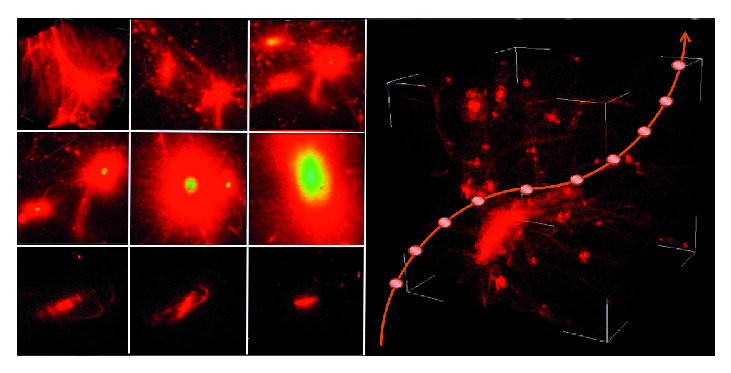
\includegraphics[scale=0.9]{part5/Massimino_O24/P024_f2}
\caption{Select frames during journey in the cosmos}
\end{figure}

\section{Computational Resources}
The required computational resources depend on the underlying hardware specification of the server. As an example, the rendering time to generate a film based on 6 player-selected frames may last up to 45 minutes. The reason is that all in-between frames are generated directly from the original cosmological simulation dataset to obtain very high quality movies.

The components of the application residing on the server will  create, between  6 snapshots, 500 frames for a total duration of the movie of 50 seconds  (10 fps). The maximum number of selectable snapshots are 18, equivalent  to a movie that lasts about 3 minutes. In this case the duration of the images generation and rendering phase is about  2 hours. The current version of the application utilizes 192MB for displaying 1 million bodies\footnote{Full dataset size: 12 GB, number of points: 500 million}. Once a movie is completed the player receives by email all necessary instructions for watching it, e.g. either by using a common browser or the application itself. Movies can also be uploaded to YouTube by using a feature of the application. Figure~3 shows the data flow of the application.

\begin{figure}[h]
\centering

\includegraphics[scale=0.9]{part5/Massimino_O24/P024_f3}
\caption{Data flow}
\end{figure}

\section{The Application}
The SpaceMission app is the first in what the developers hope will be a range of new-generation mobile tools exploiting specialized scientific data with access to DCIs to help encourage young people to become more interested in the sciences.

To this extend an interactive exhibit (supported by the Science and Technology Facilities Council, UK) based on \emph{SpaceMission} is installed at INTECH, a major science centre and planetarium in Winchester, UK. Our initial feedback is encouraging, but we are planning to formally validate \emph{SpaceMission} through a competition among high school students in the UK and Italy.

It is possible to download for free the application \emph{SpaceMission} from the iTunes Store.

Recently, the application has also being developed for Windows and MAC platforms. The packages are available for download from the official website of SpaceMission: \url{http://spacemission.oact.inaf.it}, where it is also possible to consult  all documentation and very detailed information about its features and functionalities.

\section{The sponsors}
The sponsors of the application are the Astrophysical Observatory of Catania (Italy), the Intech Science Centre and Planetarium, Winchester  (U.K.) and the University of Portsmouth (U.K.)

\acknowledgements The research leading to these results has received funding from the European Union Seventh Framework Programme (FP7/2007-2013) under grant agreement no 283481 (SCI-BUS).
